\documentclass[11pt]{article}
\renewcommand{\baselinestretch}{1.05}
\usepackage{amsmath,amsthm,verbatim,amssymb,amsfonts,amscd, graphicx}
\usepackage{graphics}
\topmargin0.0cm
\headheight0.0cm
\headsep0.0cm
\oddsidemargin0.0cm
\textheight23.0cm
\textwidth16.5cm
\footskip1.0cm
\theoremstyle{plain}
\newtheorem{theorem}{Theorem}
\newtheorem{corollary}{Corollary}
\newtheorem{lemma}{Lemma}
\newtheorem{proposition}{Proposition}
\newtheorem*{surfacecor}{Corollary 1}
\newtheorem{conjecture}{Conjecture} 
\newtheorem{question}{Question} 
\theoremstyle{definition}
\newtheorem{definition}{Definition}
\usepackage[document]{ragged2e}
\DeclareMathOperator{\Ima}{Im}
\begin{document}
 
\title{Lab 2}
\author{Zeyuan Xu}
\maketitle
\section{Task 1}
Covariance matrix is real and symmetric in this case, therefore its eigenvectors are nonzero and orthogonal vectors. Therefore they are linearly independent. So eigenvectors of $S$ form an orthogonal basis for $\mathbb{R}^d$. Therefore, a point $x_n$ in the dataset has an unique linear combination of these points. In other words, linear combination of the projection onto these vectors is unique, therefore: \begin{align*}
x_n = \sum\limits_{i=1}^{d} \langle x_n , u_i\rangle u_i  = \sum\limits_{i=1}^{d} \langle x_n - \bar{x} , u_i  \rangle u_i + \sum\limits_{i=1}^{d} \langle \bar{x} , u_i \rangle u_i = \sum\limits_{i=1}^{d} \langle x_n - \bar{x} , u_i  \rangle u_i + \bar{x}
\end{align*}
we have $\sum\limits_{i=1}^{d} \langle \bar{x} , u_i \rangle u_i = \bar{x}$,  since $\bar{x} \subset \mathbb{R}^d$, and its projection onto the same set of eigenvectors (which forms a basis for $\mathbb{R}^d$) is unique.

\section{Task 2}
By definition, projection of vector $x$ onto subspace $V$ is given by the linear combination of projection onto its basis. Since $\{ v_1, ... v_k \}$ spans $V$ and are orthonormal, it is an orthonormal basis for $\mathbb{R}^d$. Therefore we have: \begin{align*}
pV(x) = \sum\limits_{i=1}^{k} \frac{\langle x, v_i \rangle}{||v_i||^2} v_i = \sum\limits_{i=1}^{k} \langle  x, v_i \rangle v_i 
\end{align*}
as a projection to the subspace $V$. Now to show that the projection is orthogonal, This is the same to show that $pV(x)^\top p\bar{V}(y) = 0, \forall x,y \in \mathbb{R}^d$. Where $p\bar{V} (x)$ is the complement subspace of $V$, and $p\bar{V}$ represents the complement projection. We can vectorize the above expression into $pV(x) = QQ^\top x$, where $Q$ is a matrix whose column vectors are $v_1, ..., v_k$. Since $QQ^\top = I_k$, $p\bar{V}(y) = (I - QQ^\top)y$. Therefore we have that: \begin{align*}
pV(x)^\top p\bar{V}(y) &= (QQ^\top x)^\top (I-QQ^\top)y \\
&= x^\top QQ^\top y- x^\top QQ^\top QQ^\top y = 0
\end{align*}
Therefore, $pV(x)$ is an orthogonal projection of $x$ onto subspace $V$. 


\section{Task 3}
Given: \begin{align*}
& \hat{x}_n = \bar{x} + \sum\limits_{i=1}^{m} \langle x_n - \bar{x} , u_i \rangle u_i \\
& x_n = \sum\limits_{i=1}^{d} \langle x_n - \bar{x} , u_i  \rangle u_i + \bar{x}
\end{align*}
Since $\{ u_1, u_2, ..., u_d \}$ are eigenvectors of real symmetric matrix. We have that $uu^\top = I$ : \begin{align*}
J_m &= \frac{1}{N} \sum\limits_{n=1}^{N} || \hat{x}_n - x_n || ^2 \\
&= \frac{1}{N} \sum\limits_{n=1}^{N} \sum\limits_{i=m+1}^{D} ||\langle x_n - \bar{x} , u_i \rangle u_i||^2  \\
&= \frac{1}{N} \sum\limits_{n=1}^{N} \sum\limits_{i=m+1}^{D} (x^\top_n u_i - \bar{x}^\top u_i)^2 \\&= \frac{N-1}{N}\sum\limits_{i=m+1}^{D} u_i^\top S u_i\\ &= \frac{N-1}{N}\sum\limits_{i=m+1}^{D} \lambda_i 
\end{align*}


\section{Task 4}
The plot for eigenvalues of the covariance matrix $S$ for dataset is shown in figure 1: 
\begin{figure}
  \centering 
  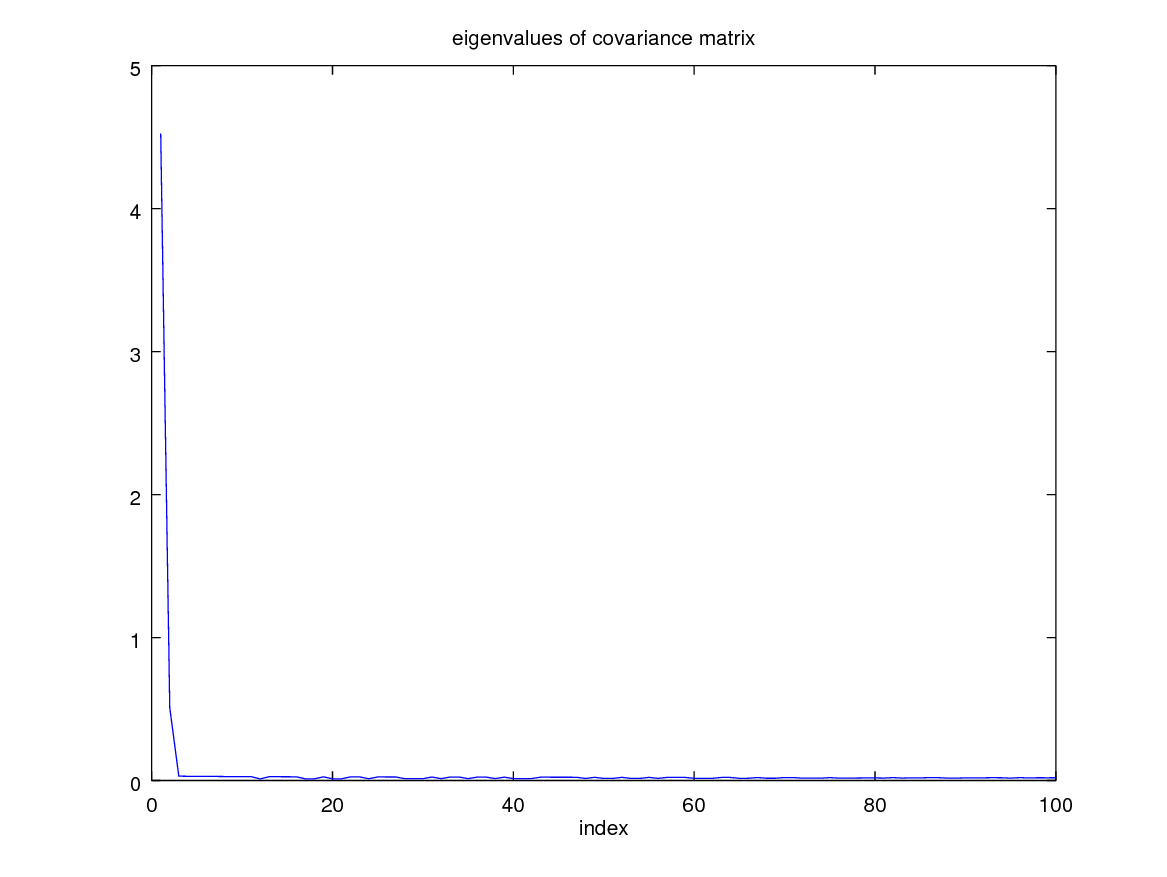
\includegraphics[width=.5\linewidth]{Task4.png}
  \caption{Eigenvalues}
  \label{fig:Eigenvalues}
\end{figure}
There is indeed a sudden drop of eigenvalues at beginning of the index. From PCA, we know that large eigenvalues of covariance matrix represent high variance, and since most of the eigenvalues are close to zero, the actual dimension of the data can be much less than 100. 

\section{Task 5}
The plot of three moon is shown in figure2. 
\begin{figure}
  \centering 
  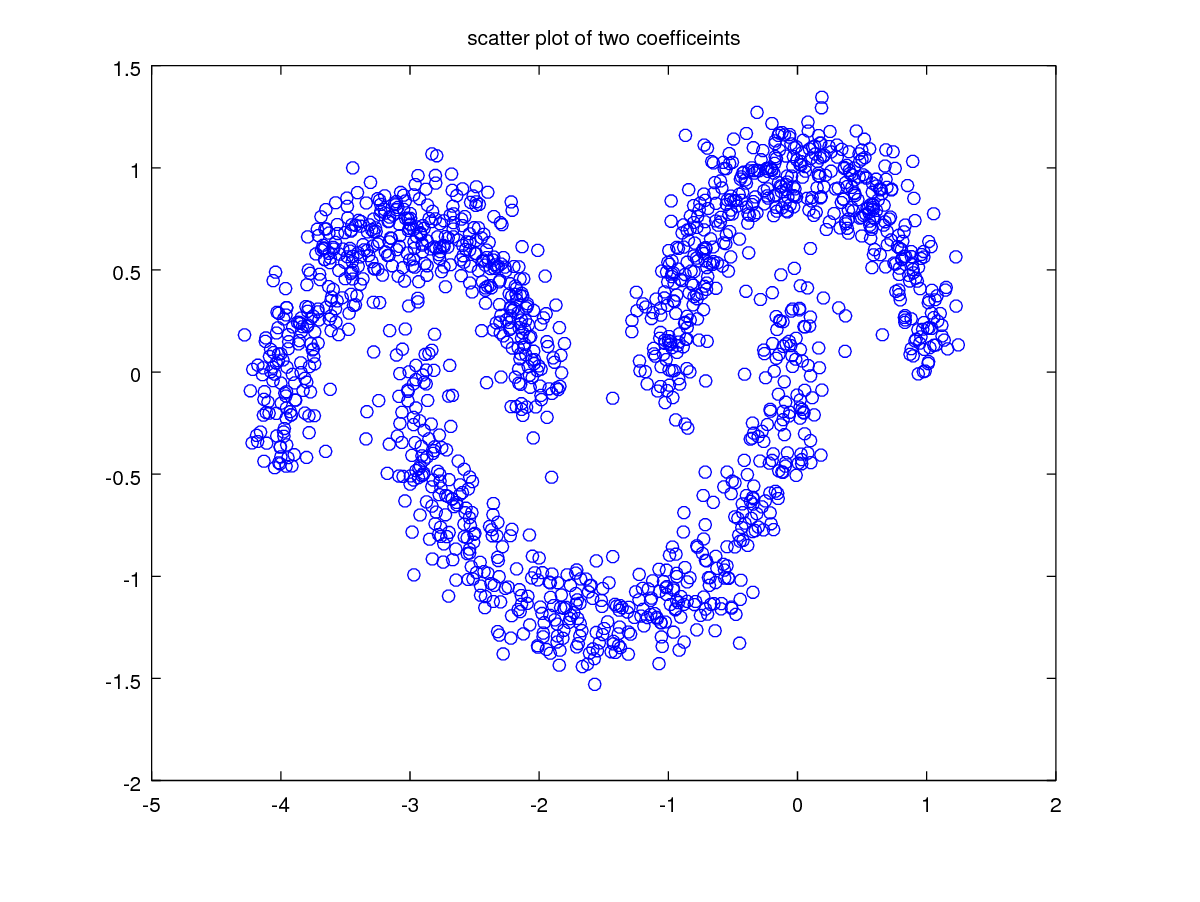
\includegraphics[width=.5\linewidth]{Task5.png}
  \caption{Three moons}
  \label{fig:Three moons}
\end{figure}

\section{Task 6} 
The original image is shown in figure 3. The plot of image rotated is shown in figure 4.

\begin{figure}[!htb]
   \begin{minipage}{0.48\textwidth}
     \centering
     
\includegraphics[width=.7\linewidth]{original.png}
     \caption{Original image}\label{Fig:Original image}
   \end{minipage}\hfill
   \begin {minipage}{0.48\textwidth}
     \centering
     
\includegraphics[width=.7\linewidth]{Task6.png}
     \caption{Rotation 90 degrees}\label{Fig:Rotate 90 degrees}
   \end{minipage}\hfill 
\end{figure} 


\section{Task 7}
Data is inherently 1-D and identified by only the rotation angle. 

\section{Task 8}
No need to compute all eigenvectors if $N < d$. Since the rank of covariance matrix is $N$.  The plot for eigenvalues of covariance matrix is shown in figure 5. 
\begin{figure}
  \centering 
  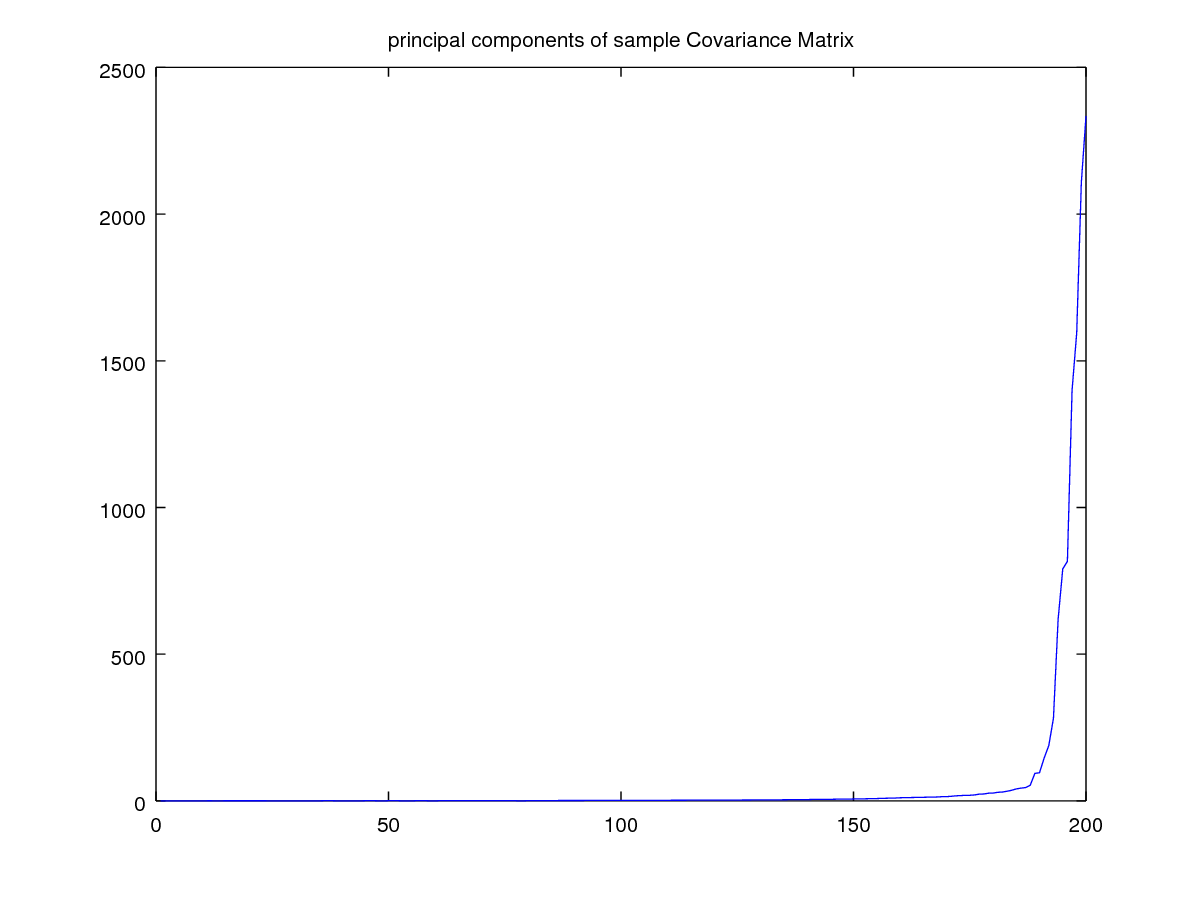
\includegraphics[width=.5\linewidth]{Task 8.png}
  \caption{Eigenvalues for Image}
  \label{fig:Eigenvalues for Image}
\end{figure}

\section{Task 9}
images for the projection onto 3 major components are in figure 6, 7, 8. The images don't make sense: they are nowhere similar to the original image, but they are suppose to be just rotations. 
\begin{figure}[!htb]
   \begin{minipage}{0.48\textwidth}
     \centering
     
\includegraphics[width=.7\linewidth]{Task9_1.png}
     \caption{First Principal Component}\label{Fig:First Principal Component}
   \end{minipage}\hfill
   \begin {minipage}{0.48\textwidth}
     \centering
     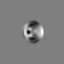
\includegraphics[width=.7\linewidth]{Task9_2.png}
     \caption{Second Principal Component}\label{Fig:Second Principal Component}
   \end{minipage}\hfill 
      \begin {minipage}{0.48\textwidth}
     \centering
     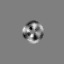
\includegraphics[width=.7\linewidth]{Task9_3.png}
     \caption{Third Principal Component}\label{Fig:Third Principal Component}
   \end{minipage}\hfill 
   \begin {minipage}{0.48\textwidth}
     \centering
     
\includegraphics[width=.7\linewidth]{Task10.png}
     \caption{Reconstruction}\label{Fig:Reconstruction}
   \end{minipage}\hfill 
\end{figure} 

\section{Task 10}
The image for using the 3 principal components to reconstruct original image is shown in figure 9. It is completely different from figure 3 (original). So it shouldn't be resonable to compress the image using only 3 principal components. 

\section{Task 11}
The image of using 198 principal components is shown in figure 10. The image of using 199 principal components is shown in figure 11. It seems that we need at least 199 principal components to reconstruct the image. Therefore, PCA is not useful for this dataset. 

\begin{figure}[!htb]
   \begin{minipage}{0.48\textwidth}
     \centering
     
\includegraphics[width=.7\linewidth]{Task11_1.png}
     \caption{198 Principal Components}\label{Fig:198 PC}
   \end{minipage}\hfill
   \begin {minipage}{0.48\textwidth}
     \centering
     
\includegraphics[width=.7\linewidth]{Task11.png}
     \caption{199 Principal Components}\label{Fig:199 PC}
   \end{minipage}\hfill 
\end{figure} 


\end{document}